\clearpage
\SourceLeaf{605}\pdfbookmark[0]{Handschriftlicher Nachlass.}{handschriftlicher-nachlass}
\thispagestyle{empty}
\vspace*{35mm}
\begin{center}
{\large HANDSCHRIFTLICHER}\par\vspace{20mm}
{\LARGE NACHLASS.}
\end{center}
\clearpage
\SourceLeaf{607}\fancyhead[L]{\small HANDSCHRIFTLICHER NACHLASS.}
\pdfbookmark[1]{Zur mathematischen Theorie der elektrodynamischen Wirkungen.}{electrodynamische-wirkungen}
\begin{center}
{\large ZUR MATHEMATISCHEN THEORIE}\par\vspace{3mm}
{\large DER ELEKTRODYNAMISCHEN WIRKUNGEN.}
\end{center}
\begin{center}[1.]\end{center}
Das allgemeine Grundgesetz für die \textit{Intensität in den einzelnen Teilen eines galvanischen Stromsystems} lässt sich auf folgende Auffassung zurückführen.

Man braucht nur Drähte gleicher Dicke zu betrachten, da man sich bei ungleicher Dicke mit der Anzahl der Drähte behelfen kann. Wäre etwa ein Draht in einem Teil $=2$, in einem anderen $=3$ dick, so könnte man dafür das System
\begin{center}\resizebox{.62\linewidth}{!}{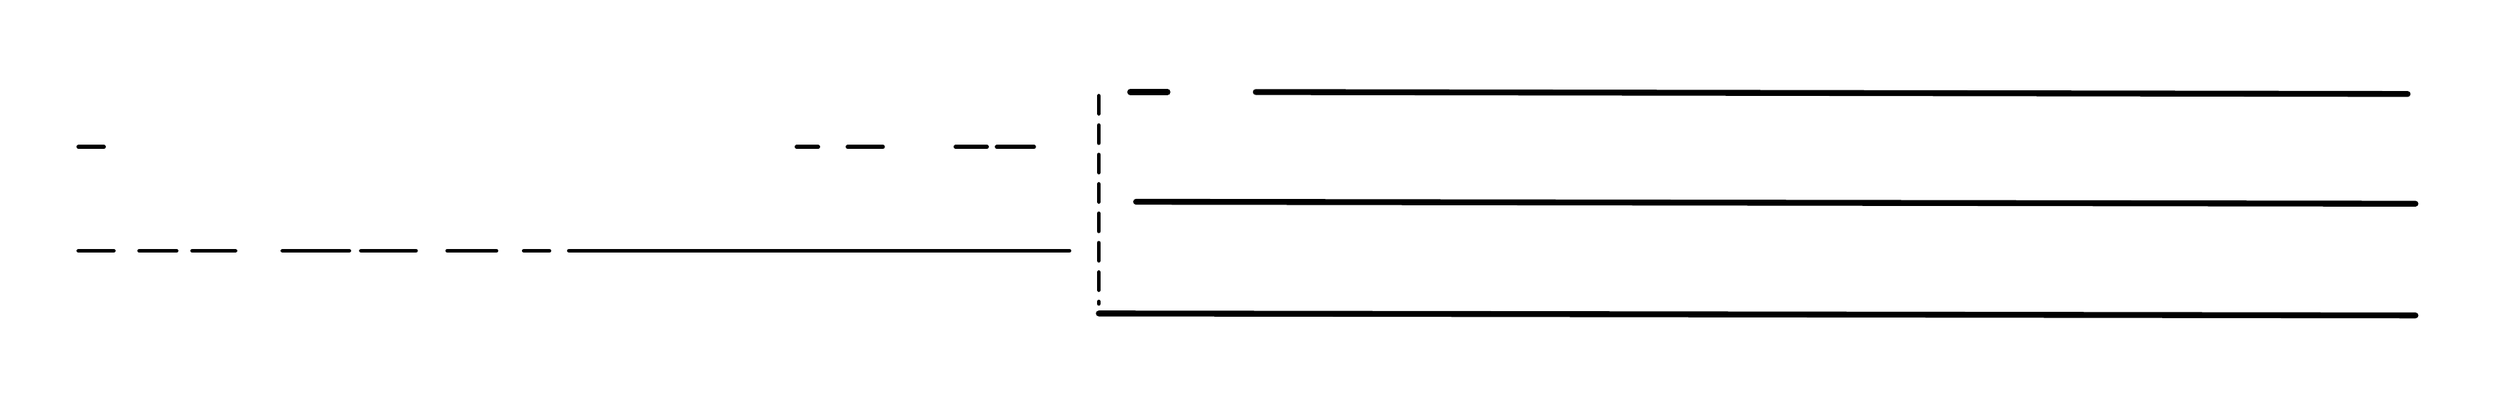
\begin{tikzpicture}[x=1bp,y=-1bp,line cap=round,line join=round]
\path[use as bounding box] (0,0) rectangle (1254,184);
\begin{pgfinterruptboundingbox}
\draw[line width=2bp] (30,65) -- (43,65);
\draw[line width=2bp] (396,65) -- (407,65);
\draw[line width=2bp] (422,65) -- (440,65);
\draw[line width=2bp] (477,65) -- (493,65);
\draw[line width=2bp] (498,65) -- (517,65);
\draw[line width=2bp] (30,118) -- (48,118);
\draw[line width=2bp] (61,118) -- (80,118);
\draw[line width=2bp] (88,118) -- (110,118);
\draw[line width=2bp] (134,118) -- (168,118);
\draw[line width=2bp] (174,118) -- (202,118);
\draw[line width=2bp] (218,118) -- (243,118);
\draw[line width=2bp] (257,118) -- (270,118);
\draw[line width=2bp] (280,118) -- (535,118);
\draw[line width=3bp] (566,37) -- (585,37);
\draw[line width=3bp] (630,37) -- (1217,38);
\draw[line width=3bp] (569,93) -- (1221,94);
\draw[line width=3bp] (550,150) -- (1221,151);
\draw[line width=2.1bp,dash pattern=on 9bp off 6bp] (550,39) -- (550,145);
\end{pgfinterruptboundingbox}
\end{tikzpicture}
}\end{center}
einsetzen.

Es geht also um die Intensität an jeder Stelle eines Systems von Linien, die wie hier zu einem Netz verbunden sind.
\begin{center}\resizebox{.63\linewidth}{!}{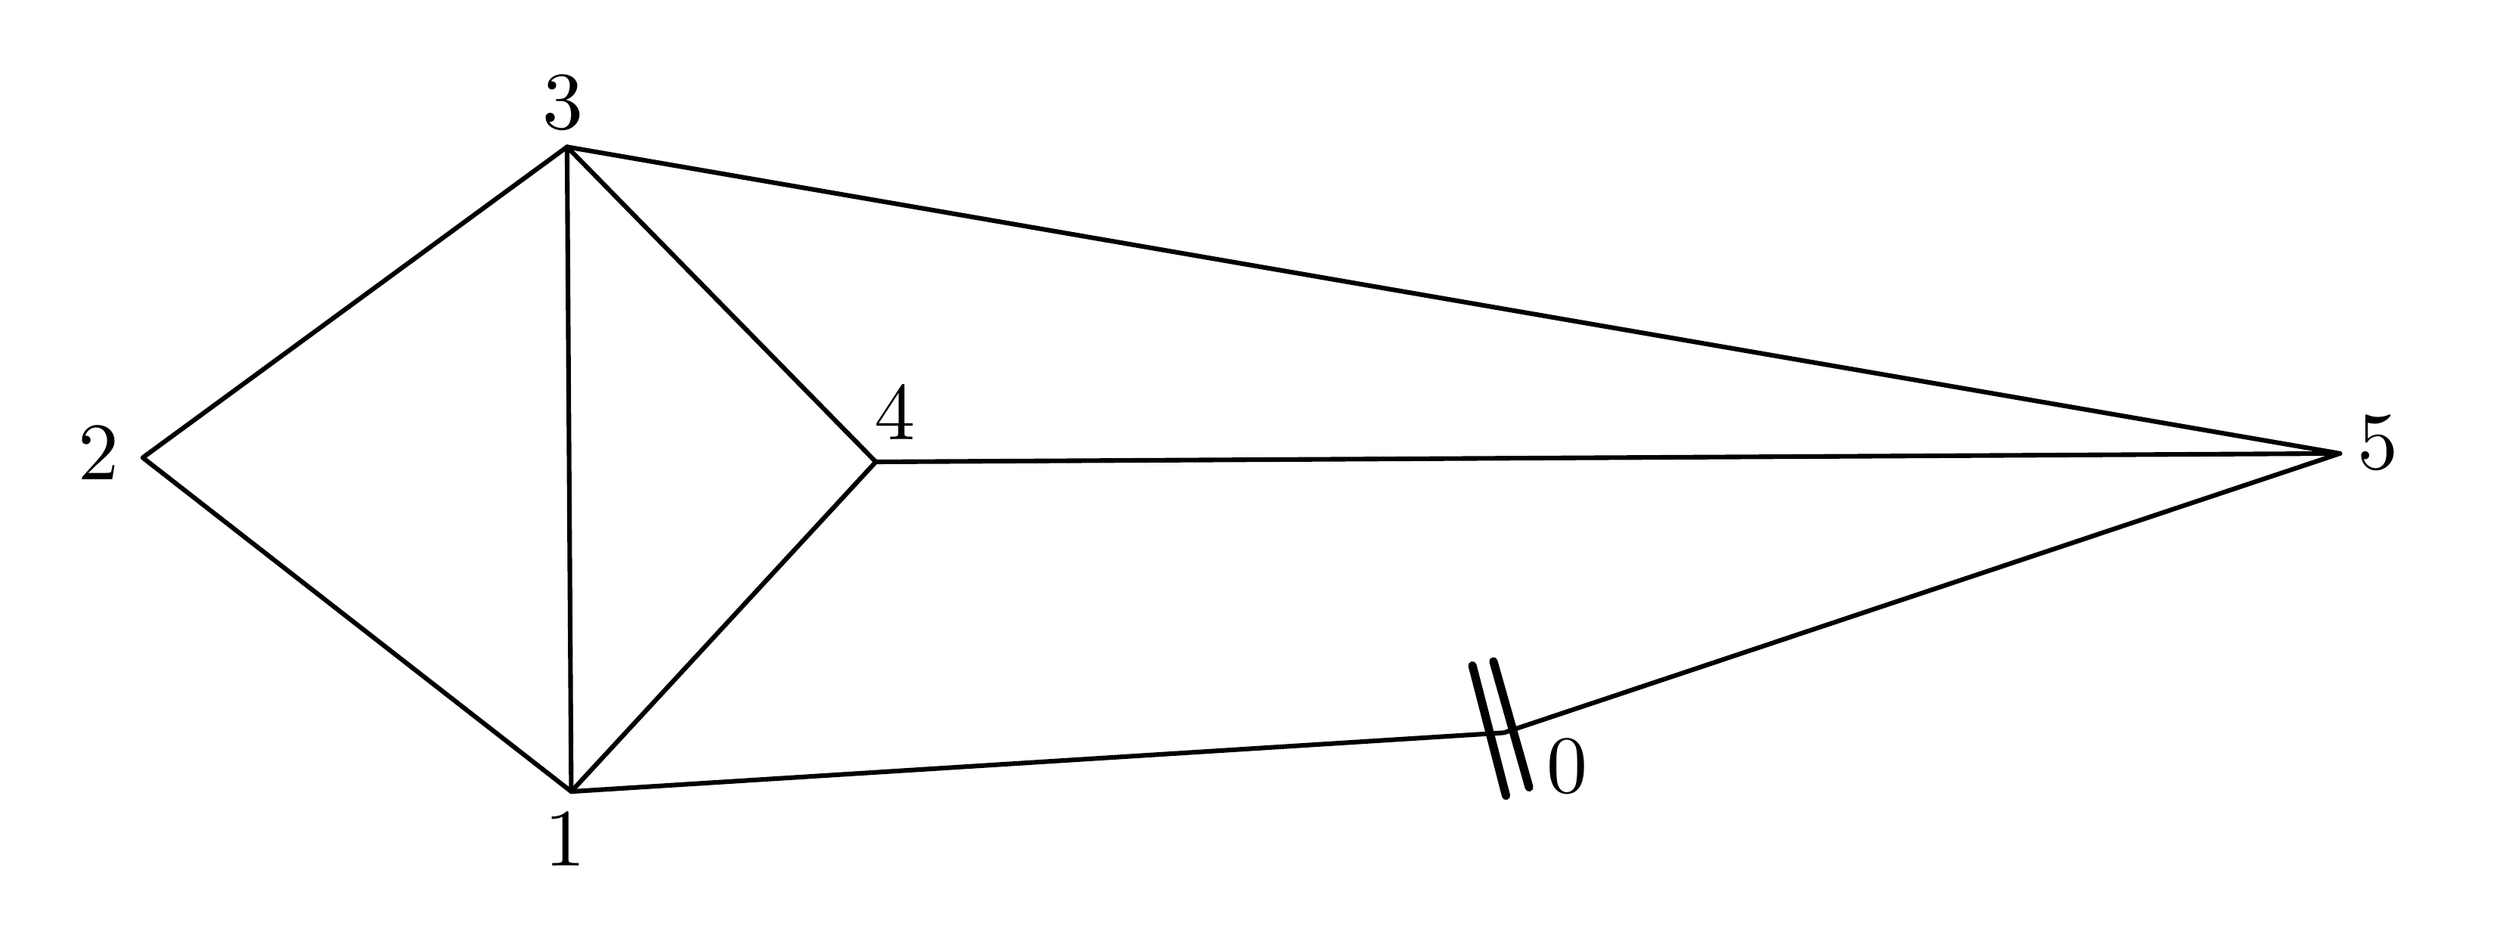
\begin{tikzpicture}[x=1bp,y=-1bp,line cap=round,line join=round]
\path[use as bounding box] (0,0) rectangle (1170,421);
\begin{pgfinterruptboundingbox}
\draw[line width=2.2bp] (262,367) -- (58,208) -- (260,60) -- (407,210) -- (262,367);
\draw[line width=2.2bp] (260,60) -- (262,367);
\draw[line width=2.2bp] (260,60) -- (1104,206) -- (407,210);
\draw[line width=2.2bp] (262,367) -- (706,339) -- (1104,206);
\draw[line width=4bp] (691,307) -- (707,369);
\draw[line width=4bp] (701,305) -- (718,365);
\node[inner sep=0pt,outer sep=0pt] at (259,390) {\scalebox{3.9}{\ensuremath{1}}};
\node[inner sep=0pt,outer sep=0pt] at (37,206) {\scalebox{3.9}{\ensuremath{2}}};
\node[inner sep=0pt,outer sep=0pt] at (258,39) {\scalebox{3.9}{\ensuremath{3}}};
\node[inner sep=0pt,outer sep=0pt] at (416,187) {\scalebox{3.9}{\ensuremath{4}}};
\node[inner sep=0pt,outer sep=0pt] at (1122,201) {\scalebox{3.9}{\ensuremath{5}}};
\node[inner sep=0pt,outer sep=0pt] at (736,355) {\scalebox{3.9}{\ensuremath{0}}};
\end{pgfinterruptboundingbox}
\end{tikzpicture}
}\end{center}
Statt aller dieser Stellen braucht man nur die Punkte zu betrachten, an denen mehr als 2 Linien zusammentreffen, sowie die Kraftsitze. Für jeden Punkt des Systems hat die Intensität \textit{einen} Wert, für die Kraftsitze hat sie \textit{zwei}.

\SourceLeaf{608}Das allgemeine Grundgesetz lautet nun so. Sei $A$ ein beliebiger Punkt, seien $A',\ A'',\ A'''\,.\,.$ Punkte, die jeweils mit $A$ einfach verbunden sind, und gebe es keinen Punkt $B$, für den weder $AB$ ein Teil einer der Verbindungen $AA',\ AA'',\ AA'''\,.\,.$ ist noch der umgekehrte Fall vorliegt. Dann hat man für jeden Punkt etwas einer Höhe Analoges anzunehmen, also $a$ im Punkt $A$, $a'$ im Punkt $A'$ und so weiter. Dann gilt stets
\[
0=\frac{a'-a}{AA'}+\frac{a''-a}{AA''}+\frac{a'''-a}{AA'''}+\,.\,.
\]
und die einzelnen Glieder dieser Summe geben stets die Stromintensität in den einzelnen Teilen an.

\vspace{3mm}
Die obige Aufgabe lässt sich allgemein wie folgt lösen. Seien $A^0,\ A^{n+1}$ die beiden Pole, $A',\ A'',\ A'''$ etc.\ $A^n$ die einzelnen Knotenpunkte des Systems und $\frac{1}{f^{\alpha,\beta}}$ der gesamte Widerstand auf dem einfachen Weg von $A^\alpha$ nach $A^\beta$. Der Nenner ist also $=0$ zu setzen, wenn zwischen den Punkten eine direkte Verbindung fehlt. Man bestimme aus den Gleichungen
\[
\begin{aligned}
(f^{1,0}+f^{1,2}+f^{1,3}+\,.\,.)p'-f^{1,0}p^0-f^{1,2}p''-f^{1,3}p'''-\text{etc.}&=0\\
(f^{2,0}+f^{2,1}+f^{2,3}+\,.\,.)p''-f^{2,0}p^0-f^{2,1}p'-f^{2,3}p'''-\text{etc.}&=0\\
(f^{3,0}+f^{3,1}+f^{3,2}+\,.\,.)p'''-f^{3,0}p^0-f^{3,1}p'-f^{3,2}p''-\text{etc.}&=0
\end{aligned}
\]
und so weiter,\quad in Verbindung mit den folgenden
\[
p^0\ \text{willkürlich},\quad p^{n+1}=p^0+k,\quad k\ \text{bezeichnet die erzeugende Kraft},
\]
die Größen $p',p'',p'''\,.\,.$. Dann ist die Stromstärke zwischen $A^\alpha$ und $A^\beta$
\[
=f^{\alpha,\beta}(p^\beta-p^\alpha)
\]

\vspace{3mm}
Das Grundprinzip lässt sich noch einfacher so darstellen.

An jedem Punkt herrscht ein \textit{bestimmter} Druck, sobald sein Wert an \textit{einem} Punkt willkürlich festgelegt ist. Zwei Sätze genügen dann, um alles in Gleichungen auszudrücken.

I.\quad Seien $A,\ B$ zwei Punkte, zwischen denen kein Knotenpunkt liegt, $P$ die Summe der Kräfte zwischen diesen Punkten, in Richtung von $A$ nach $B$ gerechnet, $\rho$ der Gesamtwiderstand zwischen diesen Punkten und $a,\ b$ die Druckwerte für diese Punkte. Dann ist $\frac{a-b+P}{\rho}=$ Intensität des Stroms in Richtung von $A$ nach $B$.

\SourceLeaf{609}II.\quad Die Summe der Intensitäten aller Ströme, von einem Punkt aus gerechnet (mehr als zwei an einem Knotenpunkt), ist $=0$.

\begin{center}[2.]\end{center}
Im Schema seien $a,b,c,d,e,f$ die Widerstände in den bezeichneten Abschnitten. Die Stromquelle liege in $a$. Ferner sei
\begin{center}\resizebox{.28\linewidth}{!}{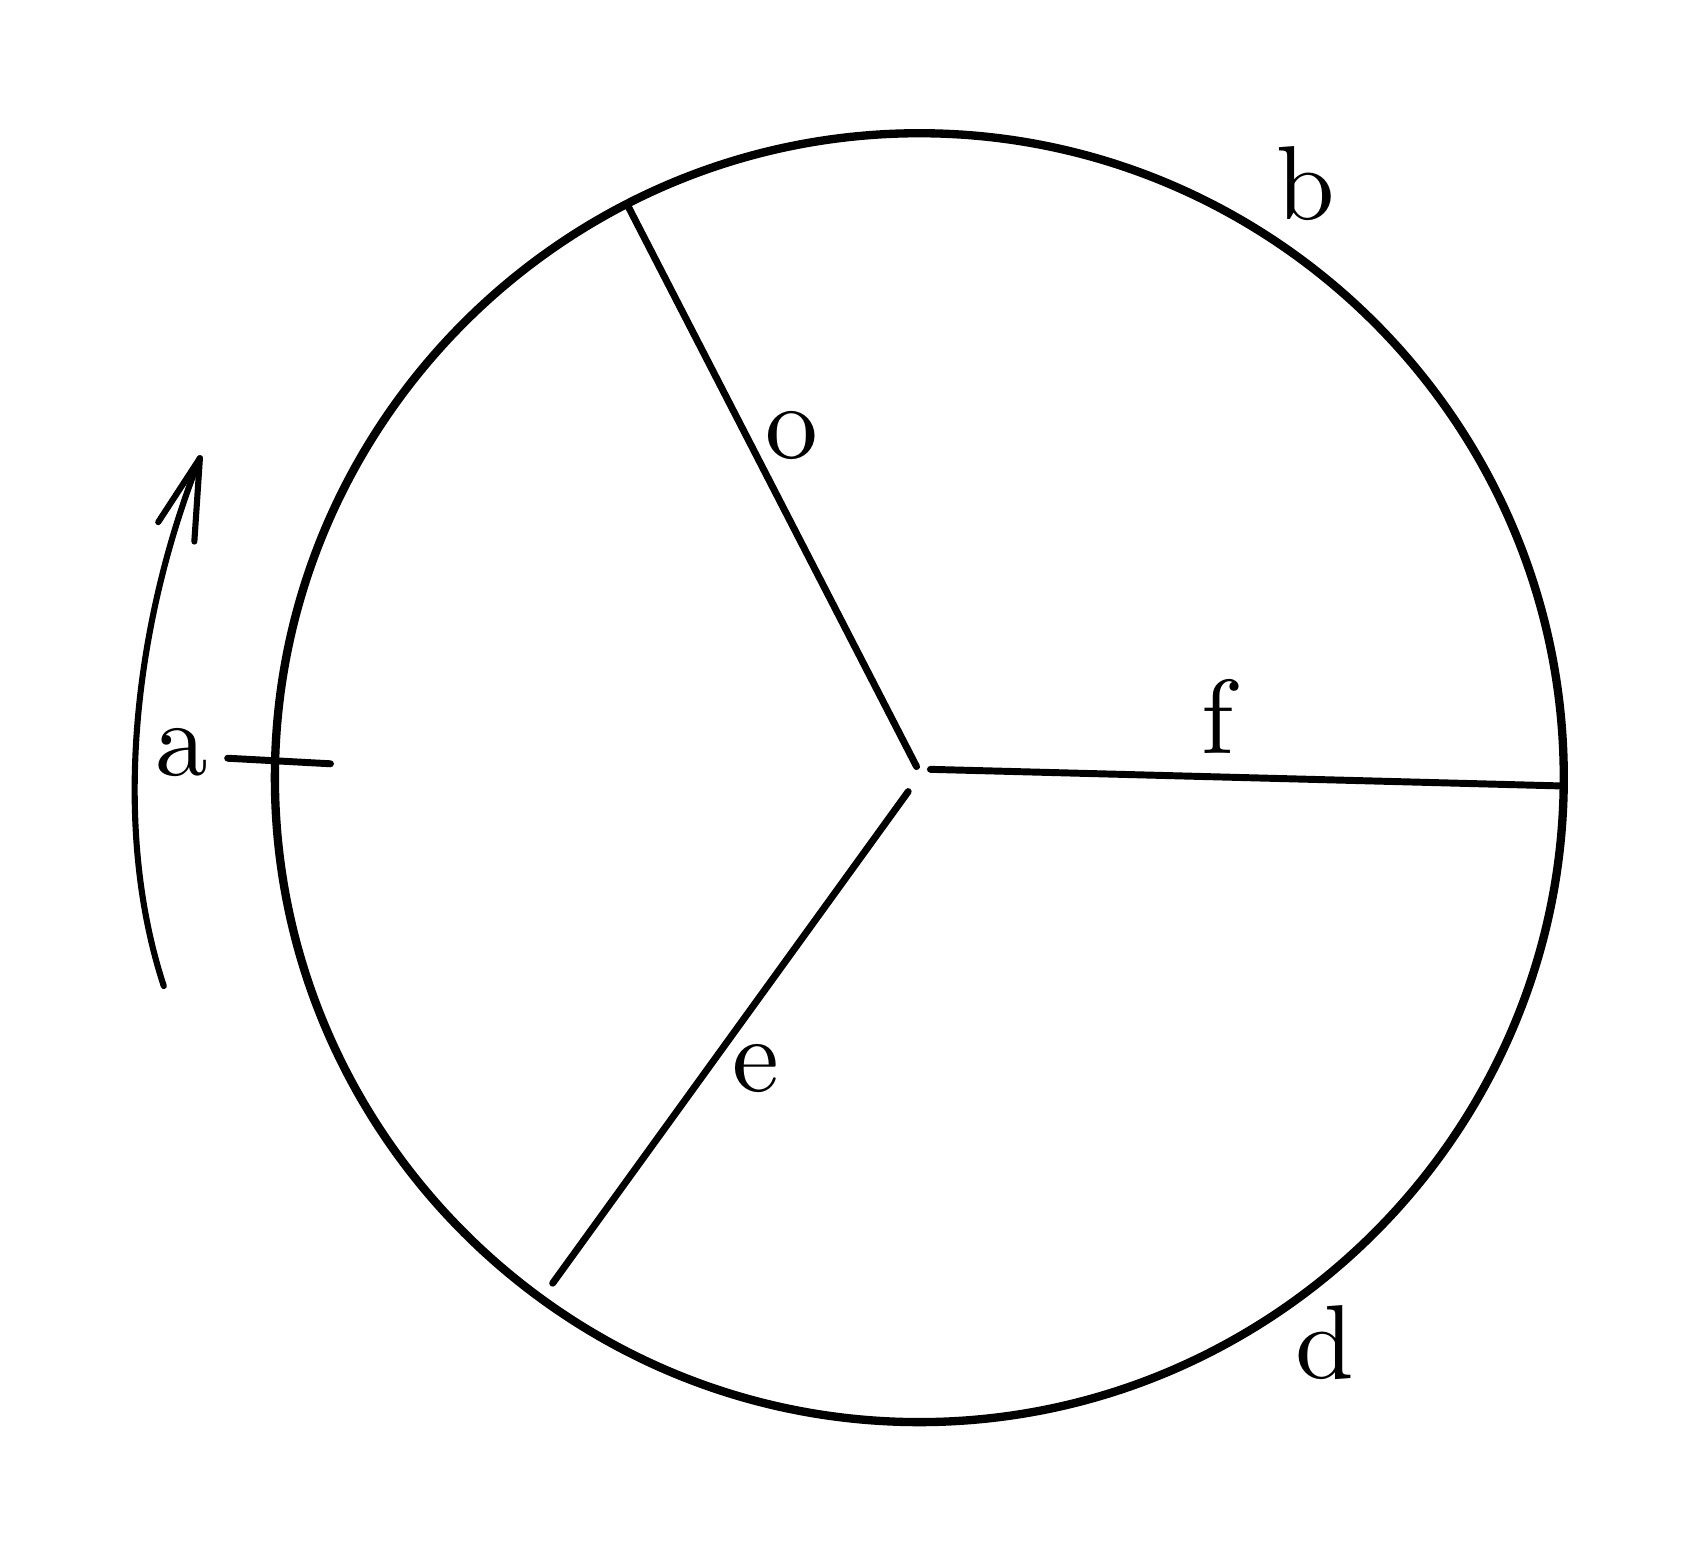
\begin{tikzpicture}[x=1bp,y=-1bp,line cap=round,line join=round]
\path[use as bounding box] (0,0) rectangle (588,535);
\begin{pgfinterruptboundingbox}
\draw[line width=3bp] (321,38) .. controls (448.60,38) and (553,142.40) .. (553,270) .. controls (553,397.60) and (448.60,502) .. (321,502) .. controls (193.40,502) and (89,397.60) .. (89,270) .. controls (89,142.40) and (193.40,38) .. (321,38);
\draw[line width=2.5bp] (216,64) -- (320,266);
\draw[line width=2.5bp] (325,267) -- (553,273);
\draw[line width=2.5bp] (317,275) -- (189,452);
\draw[line width=2.5bp] (72,263) -- (109,265);
\draw[line width=2.2bp] (49,345) .. controls (29,284) and (40,210) .. (62,155);
\draw[line width=2.2bp] (47,178) -- (62,155) -- (60,185);
\node[inner sep=0pt,outer sep=0pt] at (55,261) {\scalebox{3.8}{\ensuremath{\mathrm{a}}}};
\node[inner sep=0pt,outer sep=0pt] at (460,56) {\scalebox{3.8}{\ensuremath{\mathrm{b}}}};
\node[inner sep=0pt,outer sep=0pt] at (275,147) {\scalebox{3.8}{\ensuremath{\mathrm{o}}}};
\node[inner sep=0pt,outer sep=0pt] at (467,473) {\scalebox{3.8}{\ensuremath{\mathrm{d}}}};
\node[inner sep=0pt,outer sep=0pt] at (262,375) {\scalebox{3.8}{\ensuremath{\mathrm{e}}}};
\node[inner sep=0pt,outer sep=0pt] at (430,248) {\scalebox{3.8}{\ensuremath{\mathrm{f}}}};
\end{pgfinterruptboundingbox}
\end{tikzpicture}
}\end{center}
\[
\begin{aligned}
(b+c)(d+e)+f(b+d+c+e)&=p\\
bcde\left(\frac{1}{b}+\frac{1}{c}+\frac{1}{d}+\frac{1}{e}\right)+f(b+d)(c+e)&=q
\end{aligned}
\]
Dann ist der Gesamtwiderstand des Systems ohne den Abschnitt $a$
\[
=\frac{q}{p}
\]
und die Intensität ist
\[
\begin{aligned}
A&=\frac{(b+c)(d+e)+f(b+c+d+e)}{ap+q}=\frac{p}{ap+q}\\[4pt]
B&=\frac{cd+ce+cf+ef}{ap+q}\\[4pt]
C&=\frac{bd+be+bf+df}{ap+q}\\[4pt]
D&=\frac{be+ce+cf+ef}{ap+q}\\[4pt]
E&=\frac{bd+cd+bf+df}{ap+q}\\[4pt]
F&=\frac{be-cd}{ap+q}
\end{aligned}
\]
Aus dem Grundprinzip folgt zugleich, dass
\[
\sum rii
\]
ein Minimum sein muss, wobei $r$ den Widerstand bezeichnet, der einem Element entspricht, und $i$ die Intensität des Stroms. Noch einfacher ausgedrückt muss
\[
\sum\varepsilon vv
\]
ein Minimum annehmen, wobei $\varepsilon$ ein Element des bewegten Fluids bezeichnet und $v$ die Geschwindigkeit.

\SourceLeaf{610}Sind 0, 1, 2 etc.\ die Knotenpunkte in einem Leitungsnetz, wobei
\begin{center}\begin{tabular}{rl}
$r^{01}$ & der Widerstand\\
$i^{01}$ & die Stromstärke von 0 nach 1\\
$p^{01}$ & die bewegende Kraft von 0 nach 1 im Verbindungsstück 01\\
$q^0$ & der Druck in 0 ist\quad und so weiter, dann gilt
\end{tabular}\end{center}
\[
\begin{aligned}
\text{I.}\quad q'-q^0&=p^{01}-i^{01}r^{01}\\
\text{II.}\quad 0&=i^{01}+i^{02}+i^{03}+\text{etc.}
\end{aligned}
\]
Daraus lassen sich, wenn alle $p$ und $r$ gegeben sind, alle $q$ und $i$ bestimmen.

Sei $\Omega=\sum pi$ über alle Kombinationen. Da aus II.
\[
\sum(q'-q^0)i^{01}=0
\]
folgt, gilt
\[
\Omega=\sum iir
\]
Betrachtet man ein zweites System von Werten, in dem die $p$ unverändert bleiben und die $r$ unendlich wenig geändert sind, so gilt
\[
\begin{aligned}
\mathrm d\Omega&=\sum ii\,\mathrm dr+2\sum ir\,\mathrm di=-\sum ii\,\mathrm dr+2\sum i\,.\,\mathrm dir\\
&=-\sum ii\,\mathrm dr-2\sum i^{01}(\mathrm dq'-\mathrm dq^0)=-\sum ii\,\mathrm dr
\end{aligned}
\]
Jede Verminderung eines $r$ bei unveränderten übrigen Werten vergrößert also $\Omega$.

\begin{center}[3.]\end{center}
Die Wirkung \textit{zweier galvanischer Stromelemente} 0, 1 \textit{aufeinander} ist nach meiner Vorstellung, die übrigens erst noch weiter geprüft werden muss, die folgende.

Seien die Koordinaten der beiden Stromelemente $x,y,z$ und $x',y',z'$, Abstand $=r$. Für die Stromelemente selbst gilt $\mathrm dx=\xi$, $\mathrm dy=\eta$, $\mathrm dz=\zeta$, $\mathrm dx'=\xi'$ etc.\ Für die Wirkung, die das zweite erfährt, gilt $\delta\xi'=X'$, $\delta\eta'=Y'$ etc.\ Daraus ergibt sich
\[
\begin{aligned}
r^3X'&=\xi\{(y'-y)\eta'+(z'-z)\zeta'\}-(x'-x)(\eta\eta'+\zeta\zeta')\\
r^3Y'&=\eta\{(z'-z)\zeta'+(x'-x)\xi'\}-(y'-y)(\zeta\zeta'+\xi\xi')\\
r^3Z'&=\zeta\{(x'-x)\xi'+(y'-y)\eta'\}-(z'-z)(\xi\xi'+\eta\eta')
\end{aligned}
\]

